\chapter{Introduction}

\paragraph{Manual Overview}

This is an Operation Manual for the Kodiak Saw (BPS NNN) revised control system. Each chapter topic covers one operator screen, along with related controls and indicators. The following format is used for indicating tips \textbf{\LARGE ( \textcolor{blue}{i} )} and cautionary notes\newline \textbf{{\LARGE ( \textcolor{red}{!} )}} where necessary. As an example, the figure below shows the Main Operator Screen. Details that would follow the image of the screen shall include items of interest, such as control items and information areas, as well as status indicators. The descriptions and explanations are given from the perspective of proper equipment operation by the reader. A basic understanding of machine operation and safety procedures specific to the facility housing the equipment, should be considered a pre-requisite.
\paragraph{}
\begin{figure}
		\centering
		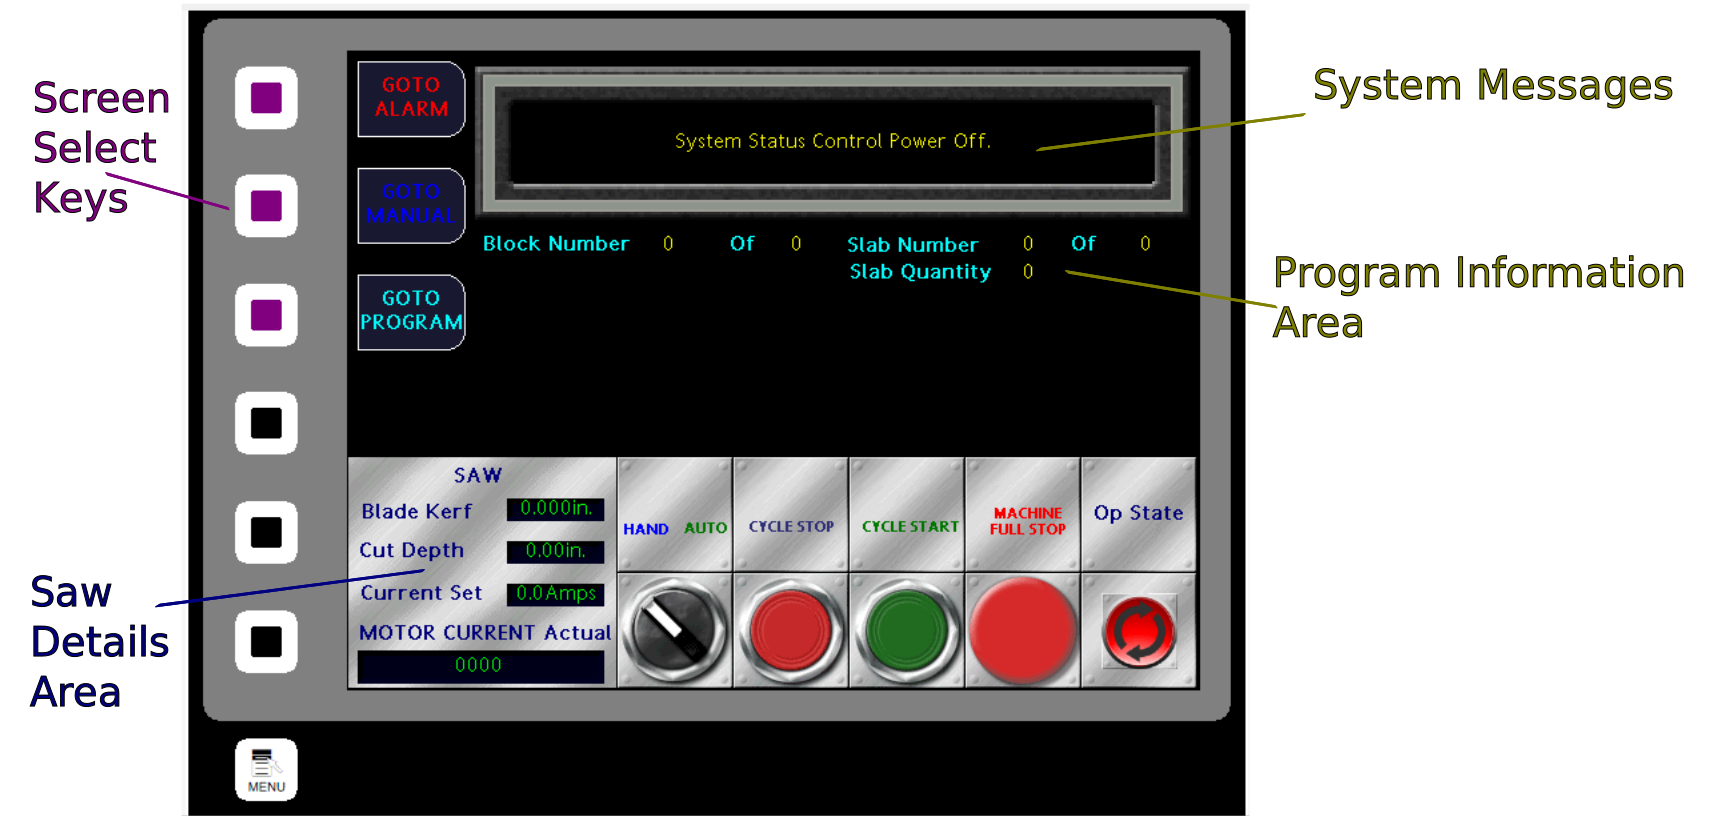
\includegraphics[width=0.5\linewidth]{screen-captures/main-screen}
		\caption{Example Screen}
		\label{fig:example-screen}
\end{figure}
\paragraph{}
\paragraph*{\textbf{\LARGE \textcolor{blue}{i}}}The Main Screen shown above, and all of the Operator Screens, use the same layout style. Navigation between screens is done using the physical buttons on the left side of the terminal, with the labels referencing what screen to goto. The operator can always return to the Main Screen from any other screen by pressing the Menu button located at the bottom left of the terminal.

\paragraph*{\textbf{{\LARGE \textcolor{red}{!}}}}A fault will be triggered by the program logic if the Operator tries to begin an Automatic Cycle without first entering a valid cut program.

\paragraph*{}
Above notes are examples of Information and Cautionary notes related to the display screen being discussed. 

\paragraph{Screen Layout Style}
 Screen navigation is done through the use of the left hand Terminal Programmable keys and the Terminal Menu key. If a Programmable Key can be used to navigate to another screen, it will be noted by a label next to that key. In the above figure of the Example Screen, there are labels next to the top three Programmable Keys. This would indicate that the Operator can navigate to the labed Screens by pressing the adjacent key. In this example, the Operator is able to navigate to either the Alarms Screen, the Manual Screen, or the Cut Program Screen. The Menu key will always return the Operator to the Main Screen from any other screen. Alarm messages and Information messages scroll through all active messages continuously until they are no longer active. Alarms are active until the Operator acknowledges them by resetting them using the Alarm Reset button on the Alarm Screen. On the Main Screen above, the Message Display Area is at the top of the Screen below the Title. The Message Area will display messages for the Operator's information, which will change according to the state of the machine. No interaction is required by the Operator since it is information only. All Alarms are displayed in the Alarm Screen Alarm Message Display Area, but indication an alarm condition exists will be displayed in the Information Display Area. Looking at the Main Screen figure above, there are control buttons located at the bottom of the screen. These are an example of how Operator Control devices and Indicator devices will be displayed and interacted with. All of the Buttons and Pilot Lights have been chosen to resemble physical Industrial Operator and Indicator devices that would normally be found on a control panel for a machine.
